\documentclass[12pt]{article}
\usepackage[serbian]{babel}
\usepackage {fontspec, amsmath, amssymb, mathtools}
\usepackage {algorithm2e, listings, alltt}
\usepackage {graphicx, float, wrapfig}

\defaultfontfeatures{Ligatures=TeX}

\addto\captionsserbian{%
  \renewcommand{\abstractname}%
    {Abstrakt}%
}

\let\oldvec\vec
\renewcommand{\vec}[1]{\mathbf{#1}}

\title{Simulacija te\v cnosti u dve dimenzije}
\author{
        Daniel Sila\dj i \\
        Gimnazija "Jovan Jovanovi\'{c} Zmaj"\\
		Novi Sad
}
\date{\today}

\begin{document}
\maketitle

\begin{abstract}
Abstrakt \ldots
\end{abstract}

\section{Uvod}\label{uvod}
    Razni fluidi su oduvek bili sastavni deo na\v sih \v zivota, pa je pored sveop\v steg razvoja tehnologije bilo pitanje vremena kad \'ce \v covek po\v zeleti da modelira i imitira njihovo kretanje, odnosno -- da ih simulira. Prirodno, i simulacije su postale deo na\v sih \v zivota, i to, sa jedne strane u vidu vremenske prognoze, aerodinami\v cki oblikovanih automobila, aviona i raketa, a sa druge strane kao specijalni efekti u filmovima i kompjuterskim igrama.

    \subsection{Istorija}\label{istorija}
        Prve korake u ovoj oblasti su napravili Claude-Louis Navier i George Gabriel Stokes 1822, postaviv\v si Navier-Stoksove jedna\v cine.
        One \v cine osnovu mnogih modela atmosfere, okeana, vodovoda, krvotoka, a koriste se i u ispitivanju aerodinami\v cnosti aviona i automobila. Ipak, ove jedna\v cine imaju jedan veliki nedostatak: ne zna se da li imaju re\v senje za proizvoljno stanje fluida u 3 dimenzije. \v Stavi\v se, to pitanje predstavlja jedan od sedam milenijumskih problema Clayovog instituta za matematiku. Zbog toga se i danas radi na pronala\v zenju \v sto br\v zih (za izra\v cunavanje), ili \v sto preciznijih aproksimacija ovih jedna\v cina, koje nam garantuju da \'ce re\v senje postojati.

        Prve kompjuterske simulacije su bile delo stru\v cnjaka iz NASA-e, ustanove koja je u tom trenutku jedina imala kompjutere dovoljno jake da simuliraju vazduh u realnom vremenu, pa makar to bilo u dve dimenzije. Bitan pomak u re\v savanju Navier-Stokesovih jedna\v cina u 3D na\v cinjen je u \cite{Foster:1996:RAL:244304.244315}, oslanjaju\'ci se na \cite{harlow:2182}.

        Osnovu ovog rada \v cini metod Smoothed Particle Hydrodynamics (SPH), otkriven 1977, nezavisno u \cite{1977MNRAS.181..375G} i \cite{1977AJ.....82.1013L}. U oba rada SPH je iskori\v s\'cen za modeliranje zvezda, i zbog toga nije pravljen da radi u realnom vremenu. Tek u \cite{Muller:2003:PFS:846276.846298} je dat pojednostavljeni algoritam, pogodan za izvr\v savanje u realnom vremenu.

    \subsection{Motivacija i cilj}\label{motivacija}
        Cilj ovog rada je simuliranje te\v cnosti u dve dimenzije, pomo\'cu metode Smoothed particle hydrodynamics, pri \v cemu je teren za simulaciju zadat od strane korisnika.

\section{Kori\v s\'cene metode}
    \subsection{Osnovni pojmovi iz dinamike fluida}
        U ovom delu je dat kratak pregled matemati\v ckih i fizi\v ckih pojmova koji se pojavljuju u Navier-Stokesovim jedna\v cinama i jedna\v cinama SPH.
        \label{definicije}
        \begin{description}
          \item[Gustina, $\rho$] predstavlja masu jedini\v cne zapremine neke supstance, odnosno $\rho = \frac{m}{V}$.
          \item[Pritisak, $p$] je skalarna veli\v cina koja je brojno jednaka sili koja deluje normalno na jedini\v cnu povr\v sinu, odnosno $p = \frac{F}{S}$
          \item[Viskozitet] je mera unutra\v snjeg trenja izme\dj u slojeva fluida. Karakteri\v se ga koeficijent viskoziteta, $\eta$.
          \item[Povr\v sinski napon] je te\v znja te\v cnosti da zauzme \v sto manju slobodnu povr\v sinu. Karakteri\v se ga koeficijent povr\v sinskog napona, $\sigma$.
              \begin{figure}[H]
              \centering%
              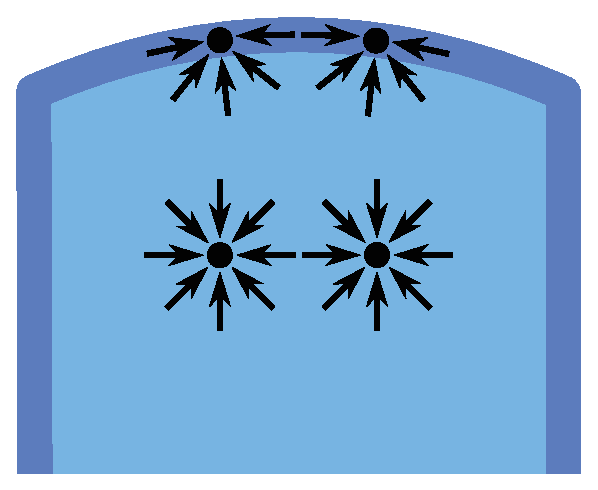
\includegraphics[width=10cm]{./figures/povrsinski_napon.eps}
              \caption{Povr\v sinski napon}
              \end{figure}
          \item[Gradijent] neke skalarne funkcije je vektorsko polje gde vektor u svakoj ta\v cki pokazuje u smeru najve\'ceg porasta, i ima intenzitet jednak tom porastu. Matemati\v cki, za funkciju $f(x, y, z)$:
                $$\nabla f=\frac{\partial f}{\partial x}\vec{i} + \frac{\partial f}{\partial y}\vec{j} + \frac{\partial f}{\partial z}\vec{k}$$ pri \v cemu se $\vec{i}, \vec{j}, \vec{k}$ jedini\v cni vektori u tri dimenzije.
                \begin{figure}[H]
                \centering%
                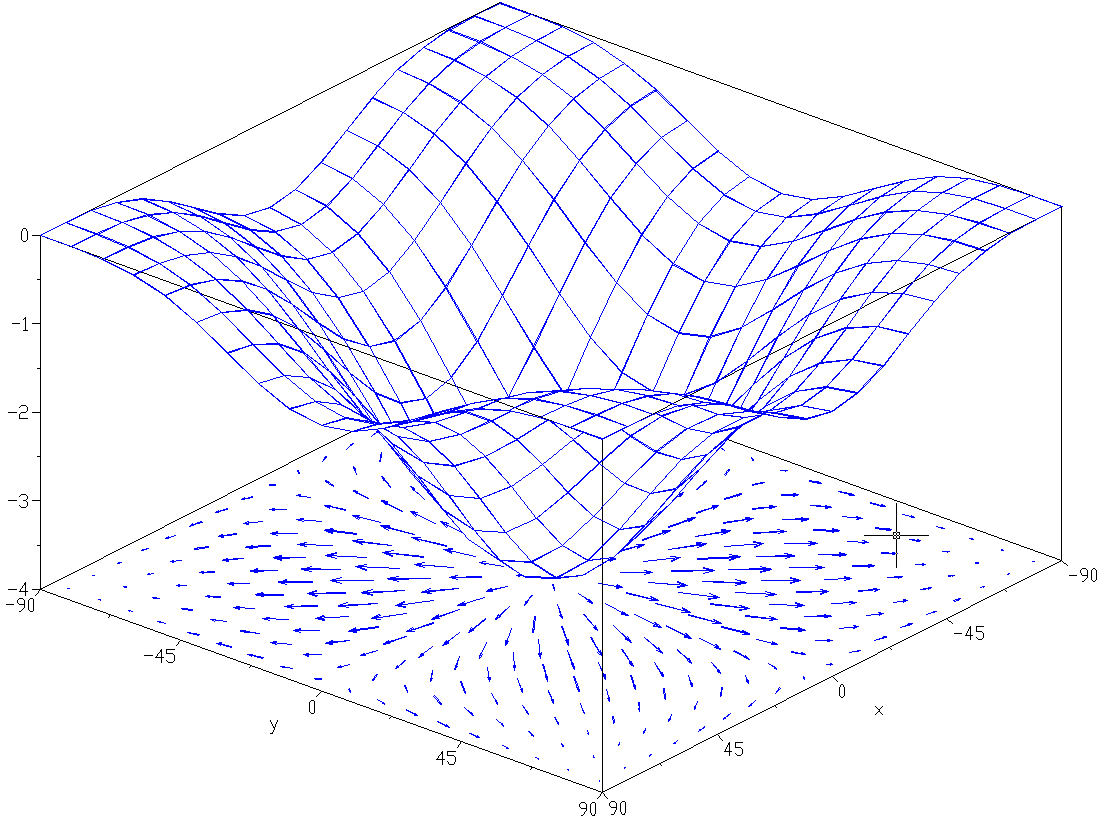
\includegraphics[width=10cm]{./figures/Gradient.png}
                \caption{Povr\v sinski napon}
                \end{figure}
          \item[Divergencija] vektorskog polja $\vec{v}(x, y, z)=v_x\vec{i}+v_y\vec{j}+v_z\vec{k}$ je skalarna funkcija
                $$\text{div} \vec{v} = \nabla \cdot \vec{v} = \frac{\partial v_x}{\partial x} + \frac{\partial v_y}{\partial y} + \frac{\partial v_z}{\partial z}$$
          \item[Laplaceov operator] funkcije $f$ je divergencija gradijenta te funkcije. $$\nabla^2 f = \nabla\cdot\nabla f = \frac{\partial^2 f}{\partial x^2} + \frac{\partial^2 f}{\partial y^2} + \frac{\partial^2 f}{\partial z^2}$$
              Za neku ta\v cku $t$, ona predstavlja meru koliko se vrednost $f$ u ta\v ckama na sferi sa centrom u $t$ menja u odnosu na $f(t)$, ako polupre\v cnik sfere raste.
        \end{description}
    \subsection{Navier-Stokesova jedna\v cina} \label{Navier Stokes}
        U op\v stem slu\v caju, Navier-Stokesova jedna\v cina izgleda ovako:
        $$ \rho(\frac{\delta \vec{v}}{\delta t} + \vec{v} \cdot \nabla \vec{v}) = -\nabla p + \nabla \cdot \vec{T} + \vec{F} $$
        Iako mo\v zda na prvi pogled deluje komplikovano, ona u stvari predstavlja drugi Newtonov zakon za kretanje fluida. Tako\dj e, za potrebe ovog rada je dovoljna pojednostavljena verzija jedna\v cine, koja se odnosi na Newtonovske fluide, nesti\v sljivog toka. Njeno izvo\dj enje sledi.

        Krenimo od dobro poznatog drugog Newtonovog zakona,
            $$\vec{F}=m\vec{a}$$
        Zamenimo ubrzanje sa materijalnim izvodom brzine po vremenu ($\vec{a} = \frac{D\vec{v}}{Dt}$), a masu sa gustinom (posmatramo jedini\v cnu zapreminu):
            $$\vec{F}=\rho\frac{D\vec{v}}{Dt}=\rho(\frac{\delta \vec{v}}{\delta t} + \vec{v} \cdot \nabla \vec{v})$$
        Sa druge strane, sile koje deluju na fluid mo\v zemo da podelimo na unutra\v snje (viskozitet, povr\v sinski napon,...) i spolja\v snje (gravitacija,...). Za po\v cetak, neka je gravitaciona sila $\rho \vec{g}$ (opet, ovo nije sila u strogom smislu te re\v ci, ve\'c sila po jedinici zapremine)
        $$\rho \vec{g} + \vec{F}_{\text{unutra\v snje}}=\rho\frac{D\vec{v}}{Dt}=\rho(\frac{\delta \vec{v}}{\delta t} + \vec{v} \cdot \nabla \vec{v})$$
        \v Sto se ti\v ce unutra\v snjih sila, radi pojednostavljivanja jedna\v cina (pa samim tim i njihovog re\v savanja), u daljem tekstu \'ce se koristiti dve pretpostavke:
        \begin{enumerate}
          \item Fluid je Newtonovski
          \item Fluid ima nesti\v sljiv tok
        \end{enumerate}
        \v Cinjenica da je fluid Newtonovski nam govori da je viskoznost konstantna, odnosno ne zavisi od tangencijalnog napona u fluidu, a iz definicije nesti\v sljivog toka znamo da je divergencija polja brzina jednaka nuli ($\nabla \cdot \vec v = 0$). Zato, unutra\v snje sile mo\v zemo podeliti na one izazvane razlikom u pritiscima (normalni napon), i na viskozne sile izazvane razlikom u brzinama (tangencijalni napon)\cite{particle-fluids}. U ovom slu\v caju, sile izazvane razlikom pritisaka mo\v zemo modelirati negativnim gradijentom pritiska ($-\nabla p$), a viskozne sile sa $\eta\nabla\cdot\nabla\vec{v}=\eta\nabla^2\vec{v}$, i tako dobijamo kona\v cnu Navier-Stokesovu jedna\v cinu za Newtonovske fluide nesti\v sljivog toka:
        $$ \underbrace{\rho}_{\text{gustina}} \overbrace{(\underbrace{\frac{\delta \vec{v}}{\delta t}}_{\text{ubrzanje deli\'ca fluida}} + \underbrace{\vec{v} \cdot \nabla \vec{v}}_{\text{konvektivno ubrzanje}})}^{\text{ubrzanje}} = \underbrace{-\nabla p}_{\text{gradijent pritiska}} + \underbrace{\eta\nabla^2\vec{v}}_{\text{viskozitet}} + \underbrace{\vec{F}}_{\text{spolja\v snje sile}} $$
    \subsection{Smoothed particle hydrodynamics}
        Osnovu SPH-a \v cini kona\v can broj \v cestica jednakih masa, od kojih svaka predstavlja jedan deo ($V_i$) zapremine datog fluida.
        Glavna prepreka u svim Lagrangeovskim algoritmima za simuliranje fluida le\v zi u \v cinjenici da je za fizi\v cki potpuno vernu simulaciju potrebno simulirati prakti\v cno neograni\v cen broj \v cestica. SPH taj problem prevazilazi tako \v sto vrednost neke fizi\v cke veli\v cine $A$ u nekoj ta\v cki $\vec{r}$ interpolira iz diskretnog skupa ta\v caka (na pozicijama $\vec{r}_i$) za koje smo ve\'c izra\v cunali vrednost $A_i$.
            $$A_\text{interpolirano}(\vec{r}) = \sum_i{A_i V_i W(\vec{r}-\vec{r}_i, h)} = \sum_i{A_i \frac{m_i}{\rho_i} W(\vec{r}-\vec{r}_i, h)}$$
        Jasno je da svaka \v cestica u\v cestvuje u $A_\text{interpolirano}$ srazmerno svojoj zapremini $V_i=\frac{m_i}{\rho_i}$ i vrednosti funkcije $W$ na udaljenosti $\vec{r}-\vec{r}_i$ od date ta\v cke $\vec{r}$ ($h$ je konstanta o kojoj \'ce uskoro biti re\v ci).

        Funkcija $W(\vec{r}, h)$ je tzv. kernel za poravnavanje (smoothing kernel) sa $h$ kao radijusom poravnavanja i slu\v zi da "rasporedi" uticaj $A_i$ u okolini (odnosno na udaljenosti $|\vec{r}-\vec{r}_i|$) \v cestice u ta\v cki $\vec{r}_i$. Zna\v caj parametra $h$ je samo u tome \v sto funkcija $W$ za vrednosti $|\vec{r}-\vec{r}_i|$ ve\'ce od $h$ ima vrednost 0, odre\dj uju\'ci preciznost simulacije tako \v sto na \v cesticu u $\vec{r}$ deluju samo \v cestice koje su joj dovoljno blizu, tj. imaju dovoljno velik uticaj na nju. Tako\dj e, radi efikasnosti i jednostavnosti simulacije, kernel se obi\v cno bira da bude simetri\v can ($W(\vec{r}, h)=W(-\vec{r}, h)$) i normalizovan ($\int W(\vec{r})d\vec{r}=1$).

        Na primer, gustina neke \v cestice se pomo\'cu gorenavedene formule mo\v ze izraziti na slede\'ci na\v cin:
        $$\rho_j=\sum_i{m_i \frac{\rho_i}{\rho_i} W(\vec{r}_j-\vec{r}_i, h)}=\sum_i{m_i W(\vec{r}_j-\vec{r}_i, h)}$$

        Da bismo mogli da izrazimo ostale \v clanove Naver Stokesove jedna\v cine, potrebni su nam oblici izraza za SPH interpolaciju za $\nabla A$ i $\nabla^2 A$. Na sre\'cu, oni se ne razlikuju mnogo od SPH izraza za interpolaciju same veli\v cine $A$:
        $$\nabla A_\text{interpolirano}(\vec{r}) = \sum_i{A_i \frac{m_i}{\rho_i} \nabla W(\vec{r}-\vec{r}_i, h)}$$
        i analogno za $\nabla^2 A$:
        $$\nabla^2 A_\text{interpolirano}(\vec{r}) = \sum_i{A_i \frac{m_i}{\rho_i} \nabla^2 W(\vec{r}-\vec{r}_i, h)}$$
        Sada imamo sve potrebne ''alate'' da izvedemo SPH jedna\v cine za ostale \v clanove Navier Stokesove jedna\v cine.
        \subsubsection{Pritisak}
            Koriste\'ci SPH interpolaciju, izraz za ''sile pritiska'' izgleda ovako:
            $$\vec{F}_{\text{pritisak}_i} = -\nabla p(\vec{r}_i)=-\sum_j p_j \frac{m_j}{\rho_j}\nabla W(\vec{r}_i-\vec{r}_j, h)$$
            Na\v zalost, ovakav izraz za silu pritiska nije simetri\v can, tj. sila kojom \v cestica $i$ deluje na \v cesticu $j$ je razli\v cita od sile kojom \v cestica $j$ deluje na \v cesticu $i$ . Zato, u \cite{Desbrun96smoothedparticles:} je predlo\v zena jednostavna metoda kako da se prethodna jedna\v cina simetrizuje: gustina $\rho_j$ se zameni sa aritmeti\v ckom sredinom gustina $\rho_i$ i $\rho_j$:
            $$\vec{F}_{\text{pritisak}_i} = -\sum_j m_j \frac{p_i+p_j}{2\rho_j}\nabla W(\vec{r}_i-\vec{r}_j, h)$$
            Jedino ostaje kako izra\v cunati pritiske kod \v cestica $i$ i $j$, a odgovor na njega je dat u \cite{Muller:2003:PFS:846276.846298}, inspirisan osnovnom jedna\v cinom gasnog stanja za idealni gas pri konstantnoj temperaturi:
            $$p = k(\rho-\rho_0)$$
            $\rho_0$ je konstanta nazvana ''gustina ostatka'' (rest density), i ne\'ce uticati na rezultuju\'ce sile (koje se zasnivaju na razlici pritisaka), ali \'ce zato (pozitivno) uticati na numeri\v cku stabilnost simulacije \cite{Muller:2003:PFS:846276.846298}.
        \subsubsection{Viskozne sile}
            Analogno izrazu za sile pritiska, dobijamo:
            $$\vec{F}_{\text{viskozitet}_i} = \eta\nabla^2 \vec{v}(\vec{r}_i)=\eta\sum_j \vec{v}_j \frac{m_j}{\rho_j}\nabla^2 W(\vec{r}_i-\vec{r}_j, h)$$
            Ni ova jedna\v cina ne daje simetri\v cne sile izmedju \v cestica $i$ i $j$, pa je balansiramo zamenjivanjem $\vec{v}_j$ sa $\vec{v}_j-\vec{v}_i$, odnosno $\vec{v}_i-\vec{v}_j$:
            $$\vec{F}_{\text{viskozitet}_i}=\eta\sum_j m_j \frac{\vec{v}_j-\vec{v}_i}{\rho_j}\nabla^2 W(\vec{r}_i-\vec{r}_j, h)$$
            Ova smena je sa fizi\v cke ta\v cke gledi\v sta sasvim opravdana, jer viskozne sile zavise od relativnih brzina slojeva te\v cnosti, a ne njihove apsolutne vrednosti.
        \subsubsection{Povr\v sinski napon}
            Radi vernije simulacije te\v cnosti, potrebno je uvesti i silu povr\v sinskog napona, koja je odgovorna za razne pojave uklju\v cuju\'ci ''barice'' koje nastaju pri prosipanju te\v cnosti na neku podlogu, kapilarne efekte, ... Prirodno, da bismo izra\v cunali povr\v sinski napon, potrebno je prvo odrediti koje \v cestice su najbli\v ze povr\v sini. To se posti\v ze metodom ''polja boja'' (colour field), koja u ta\v ckama gde se nalaze \v cestice ima vrednost 1, a u ostalim 0. Naravno, ovakvo polje je nepogodno za rad, pa se zato koristi njegova poravnata varijanta, sli\v cna ostalim SPH formulama:
            $$c_S(\vec{r}) = \sum_i 1\cdot\frac{m_i}{\rho_i}W(\vec{r}-\vec{r}_i, h)$$
            Sada se vidi da \'ce ovakvo polje imati velik gradijent blizu povr\v sine (mnogo prelaza iz 1 u 0), i mali u unutra\v snjosti te\v cnosti (uglavnom vrednosti blizu 1). Po\v sto u povr\v sinskom naponu u\v cestvuje i zakrivljenost slobodne povr\v sine te\v cnosti, potrebno je izraziti i taj ugao zakrivljenosti:
            $$\kappa = \frac{-\nabla^2c_S}{|\nabla c_S|}$$
            Kombinuju\'ci ove jedna\v cine, dobijamo:
            $$\vec{F}_{\text{pov. napon}} = \sigma\kappa\nabla c_S = -\sigma \nabla c_S \frac{\nabla^2 c_S}{|\nabla c_S|}$$
        \subsubsection{Dodatne napomene}
            Kao \v sto je ve\'c nagove\v steno na po\v cetku dela \ref{Navier Stokes}, po\v sto se u SPH posmatraju nesti\v sljive \v cestice, mo\v zemo zanemariti advekciju, odnosno $\nabla \cdot \vec{v}=0$, Navier Stokesova jedna\v cina za ovakve \v cestice je:
            $$\rho \frac{\partial \vec{v}}{\partial t} = -\nabla p +\eta \nabla^2\vec{v}+\vec{F}$$.
    \subsection{Interakcija sa \v cvrstim telima}
        Interakcija sa \v cvrstim telima (u daljem tekstu: zidovima) je re\v sena na dva na\v cina: SPH i sudar \v cvrstih tela.
        \subsubsection{SPH na\v cin}
            Iako ova metoda nije opisana nigde u literaturi, do nje se prirodno dolazi primenom SPH logike: zidovi se posmatraju kao da su i sami napravljeni od stati\v cnih \v cestica velike gustine. Naravno, ovakav na\v cin predstavljanja nije zgodan ni za ljudsku, ni za kompjutersku upotrebu. Zato, ljudi (korisnici) unose linije kao parove ta\v caka, a program implicitno pravi nove \v cestice u blizini podno\v zja normale iz \v cestice na zid. Zatim se te \v cestice zida normalno koriste u SPH jedna\v cinama za ra\v cunanje gustina, i sila koje deluju na \v cestice te\v cnosti. Prirodno, nisu nam bitne sile koje deluju na \v cestice zida, jer je pretpostavka da je zid stati\v can.
        \subsubsection{Sudar \v cvrstih tela}
            Sa druge strane, ako i posle primene prethodnog algoritma postoji opasnost da \v cestica pro\dj e kroz zid, ovaj primitivni algoritam \'ce je odbiti kao gumenu lopticu, reflektovanjem vektora njene brzine u odnosu na zid. Ovo je poslednji deo svakog koraka simulacije, i izvr\v sava se sve dok tokom simuliranog vremena ($dt$) \v cestica ima u blizini zid kroz koji bi pro\v sla, a da nije prethodno bila odbijena od njega.
    \subsection{Simulacija}
        \subsubsection{Pseudokod}
        \lstset{breaklines=true}
            \begin{lstlisting}
dokle god simulacija radi
{
    za svaki par cestica {p1, p2} izracunati gustine koje one jedna drugoj dodaju
    za svaku cesticu p i svaki zid z izracunati dodatnu gustinu za cesticu p
    za svaki par cestica {p1, p2} izracunati dodatne sile pritisaka, viskozne sile, gradijent polja boja, Laplasov operator polja boja
    za svaku cesticu p i svaki zid z izracunati dodatnu silu pritiska i viskoziteta
    za svaku cesticu p izracunati sile povrsinskog napona
    za svaku cesticu p izracunati ukupnu silu, ubrzanje, novu brzinu i pomeraj
    svaku cesticu p odbijati od prepreka, kao sto je opisano u delu 2.4.2
}
            \end{lstlisting}
        \subsubsection{Tehi\v cki detalji}
            Program je pisan u programskom jeziku C++. Za grafiku je kori\v s\'cena biblioteka SDL, koja se oslanja na OpenGL grafi\v cki sistem.
            Teren za simulaciju, kao i ostali parametri simulaciju su sa\v cuvani u JSON formatu, za \v cije je u\v citavanje kori\v s\'cena biblioteka Boost.
    \section{Rezultati}
        OVDE DOLAZE REZULTATI!
\newpage
\bibliographystyle{abbrv}
\bibliography{2DSPH}

\end{document}
This is never printed
